\documentclass{standalone}
\usepackage{amssymb,amsmath}
\usepackage{tikz}
\usetikzlibrary{automata,positioning}
\begin{document}
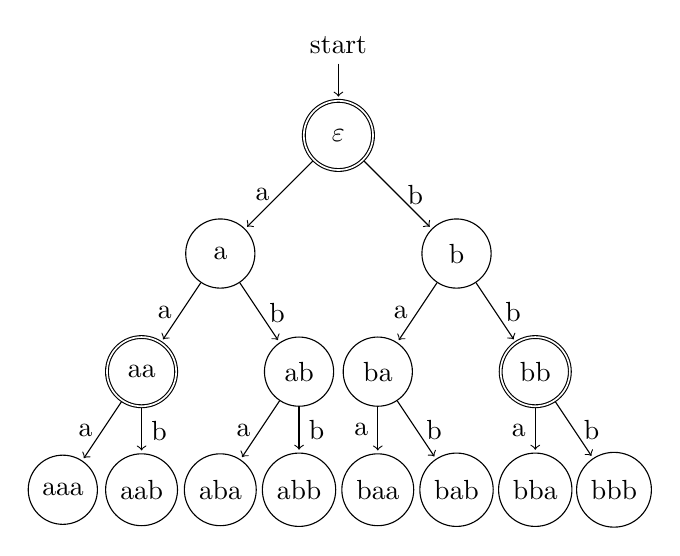
\begin{tikzpicture}[shorten >=1pt,node distance=2cm,on grid,auto] 
 \node[state,initial above,accepting] (s_0) {$\varepsilon$};
 \node[state] (s_a) at (-1.5,-1.5) {a};
 \node[state] (s_b) at (1.5,-1.5) {b};
 \node[state,accepting] (s_aa) at (-2.5,-3.0) {aa};
 \node[state] (s_ab) at (-0.5,-3.0) {ab};
 \node[state] (s_ba) at (0.5,-3.0) {ba};
 \node[state,accepting] (s_bb) at (2.5,-3.0) {bb};
 \node[state] (s_aaa) at (-3.5,-4.5) {aaa};
 \node[state] (s_aab) at (-2.5,-4.5) {aab};
 \node[state] (s_aba) at (-1.5,-4.5) {aba};
 \node[state] (s_abb) at (-0.5,-4.5) {abb};
 \node[state] (s_baa) at (0.5,-4.5) {baa};
 \node[state] (s_bab) at (1.5,-4.5) {bab};
 \node[state] (s_bba) at (2.5,-4.5) {bba};
 \node[state] (s_bbb) at (3.5,-4.5) {bbb};

 \path[->] 
 (s_0) edge [left] node {a} (s_a)
 (s_0) edge [right] node {b} (s_b)
 (s_a) edge [left] node {a} (s_aa)
 (s_a) edge [right] node {b} (s_ab)
 (s_b) edge [left] node {a} (s_ba)
 (s_b) edge [right] node {b} (s_bb)
 (s_aa) edge [left] node {a} (s_aaa)
 (s_aa) edge [right] node {b} (s_aab)
 (s_ab) edge [left] node {a} (s_aba)
 (s_ab) edge [right] node {b} (s_abb)
 (s_ba) edge [left] node {a} (s_baa)
 (s_ba) edge [right] node {b} (s_bab)
 (s_bb) edge [left] node {a} (s_bba)
 (s_bb) edge [right] node {b} (s_bbb);
\end{tikzpicture} 
 \end{document}